\documentclass[12pt, a4paper]{ctexart}

% --- 1. 基础结构与排版宏包 (必须在 unicode-math 之前加载) ---
\usepackage{amsmath}
\usepackage{graphicx}
\usepackage{geometry}
\usepackage{listings}
\usepackage{xcolor}
\usepackage{float}

\geometry{left=2.5cm, right=2.5cm, top=2.5cm, bottom=2.5cm}

% --- 2. 完美字体配置 ---
\usepackage{fontspec}
\usepackage{unicode-math}

% 英文正文：调用系统中的 Times New Roman
\setmainfont{times.ttf}[
    BoldFont = timesbd.ttf,
    ItalicFont = timesi.ttf,
    BoldItalicFont = timesbi.ttf
]

% 中文正文：强制指定系统中安装的宋体，并允许伪粗体和伪斜体
\setCJKmainfont{simsun.ttc}[
    AutoFakeBold = true,
    AutoFakeSlant = true
]

% 数学公式：调用 TeX Live 自带的顶级 Times 风格数学字体 (纯正 MathType 质感)
\setmathfont{texgyretermes-math.otf}

% --- 3. Python 代码高亮设置 ---
\lstset{
    language=Python,
    basicstyle=\ttfamily\footnotesize,
    keywordstyle=\color{blue},
    stringstyle=\color{red},
    commentstyle=\color{green!60!black},
    numbers=left,
    numberstyle=\tiny\color{gray},
    stepnumber=1,
    frame=single,
    breaklines=true
}

\title{\textbf{自适应 Hopf 振荡器：动态频率学习机制与耦合强度影响分析}}

\date{}

\begin{document}

\maketitle

\section{基础 Hopf 振荡器模型}

在机器人 CPG（中枢模式发生器）控制中，
最基础的数学表达为孤立的 Hopf 振荡器。
在笛卡尔坐标系下，其微分方程组如下：

\begin{equation}
    \begin{cases}
        \dot{x} = \gamma(\mu - x^2 - y^2)x - \omega y \\
        \dot{y} = \gamma(\mu - x^2 - y^2)y + \omega x
    \end{cases}
\end{equation}

其中，$x, y$ 为系统状态变量（$x$ 常映射为关节期望位置），$\gamma$ 为恢复系数，$\mu$ 决定了极限环的振幅（$\sqrt{\mu}$），常数 $\omega$ 为系统的固有频率 。该系统能在相平面上产生极其稳定、具有拓扑鲁棒性的极限环 。

% --- 预留插图位置 1 ---
\begin{figure}[htbp]
    \centering
    % 把宽度的比例调大，比如 0.95\textwidth
    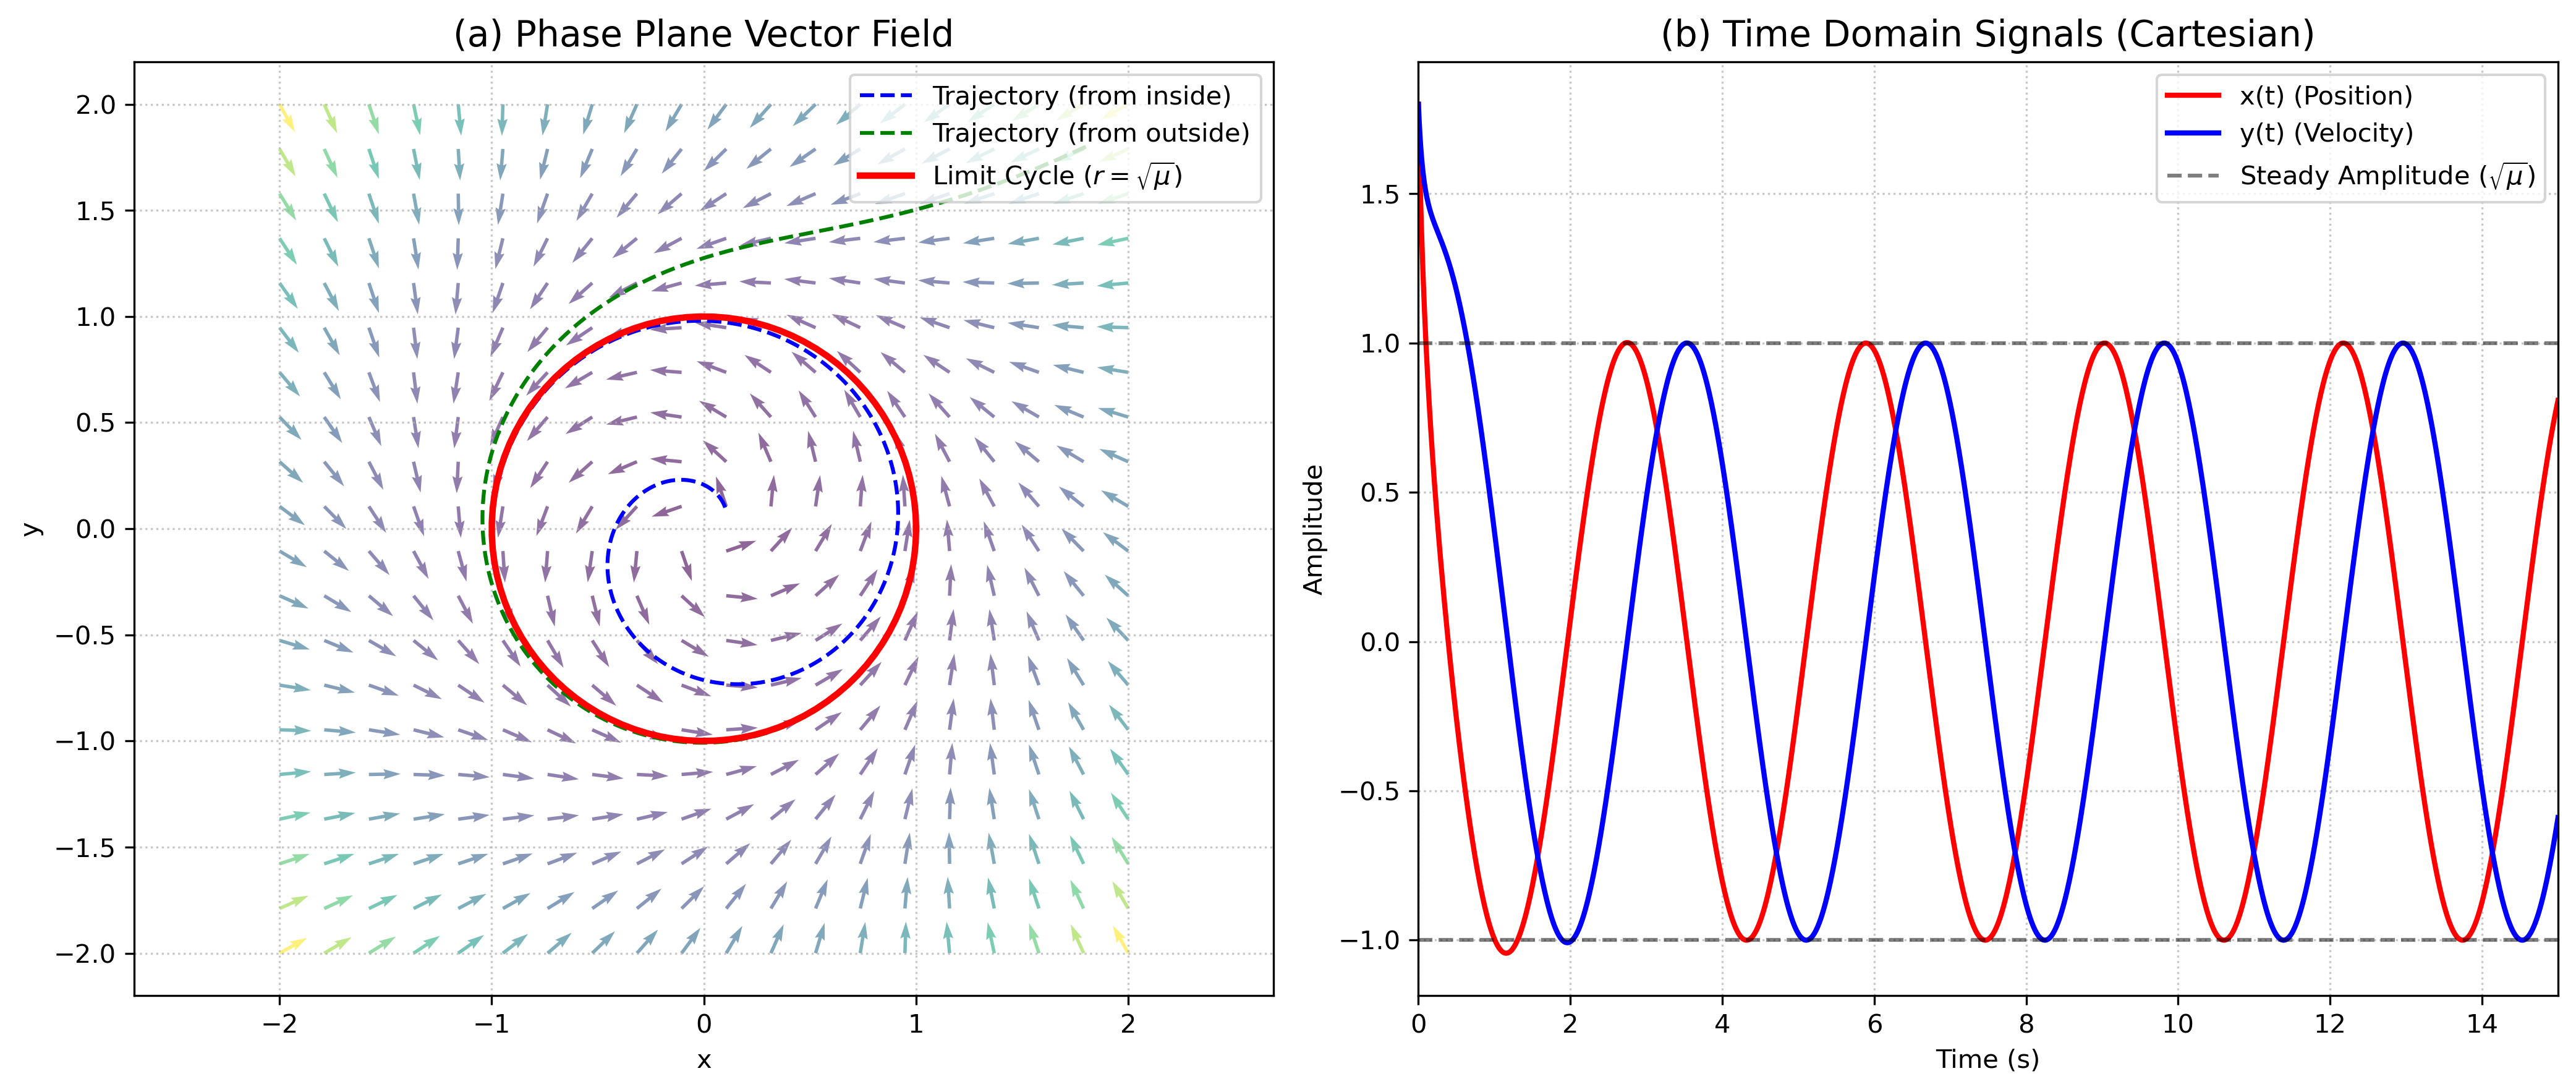
\includegraphics[width=0.95\textwidth]{figure/figure_source/figure1_limit_cycle.png} 
    \caption{基础 Hopf 振荡器的动态特性：(a) 相平面上的极限环矢量场；(b) 笛卡尔坐标系下的状态变量时域演化}
    \label{fig:basic_hopf}
\end{figure}

\section{自适应频率学习机制}

为了使机器人在复杂地形（如受扰动、物理共振频率改变）下能够自适应地调整步频，引入外部物理交互力 $F(t)$，并将频率 $\omega$ 升级为状态变量，引入动态赫布学习（Dynamic Hebbian Learning）法则：

\begin{equation}
    \begin{cases}
        \dot{x} = \gamma(\mu - r^2)x - \omega y + \varepsilon F(t) \\
        \dot{y} = \gamma(\mu - r^2)y + \omega x \\
        \dot{\omega} = -\varepsilon F(t) \frac{y}{r}
    \end{cases}
\end{equation}

其中，$r = \sqrt{x^2+y^2}$，$\varepsilon$ 为耦合强度（Coupling Strength），决定了 CPG 对外部扰动信号的敏感程度。

\textbf{耦合项 $\varepsilon F(t)$ 的动力学机理与核心作用：}

在自适应 CPG 控制中，外部物理反馈 $\varepsilon F(t)$ 扮演着连接“内部控制节律”与“外部物理世界”的关键桥梁，主要实现以下两个核心功能：

\begin{itemize}
    \item \textbf{驱动相位锁定 (Phase Locking)：} 在机器人实际运动（如步行或弹跳）中，如果内部 CPG 生成的关节参考轨迹 $x(t)$ 与地面反作用力 $F(t)$ 的节奏不匹配，就会导致“踩空”或“对抗发力”。方程 $\dot{x}$ 中的 $\varepsilon F(t)$ 相当于一个\textbf{动态校准器}。当内外节律出现偏差时，该项会实时对 CPG 的状态施加补偿——如果 CPG 跑得比物理环境快，它就产生阻力“拽”住状态；如果跑得慢，就产生推力“催”促状态。最终，它会强制 CPG 的输出波形与外部物理反馈保持稳定的、恒定的时间差，实现完美的动作协同（即相位锁定）。
    
    \item \textbf{主导频率自适应演化 (Frequency Adaptation)：} 机器人在不同地形或携带不同负载时，其最佳机械共振频率是未知的。方程 $\dot{\omega}$ 中的 $-\varepsilon F(t) \frac{y}{r}$ 项实现了一种在线学习机制。从信号处理的角度看，它本质上是在计算外部物理反馈与内部振荡节律的\textbf{相关性偏差}。当内外频率不一致时，该项会持续累积误差，驱动内部期望频率 $\omega$ 发生自动上调或下调；一旦系统与环境达到上述的“相位锁定”状态，该偏差项的宏观均值就会归零，使 $\omega$ 精准且平滑地稳定在当前环境的真实物理节律上。
\end{itemize}

如图 \ref{fig:entrainment_mechanism} 所示，在耦合项的驱动下，系统不仅在时域波形上迅速完成了与外部激励的相位重合，其内部控制参数 $\omega$ 也实现了向环境动力学特征的收敛。这种机制在底层控制律层面，赋予了机器人应对复杂外部扰动的自适应能力。

% --- 新增插图位置 ---
\begin{figure}[H]
    \centering
    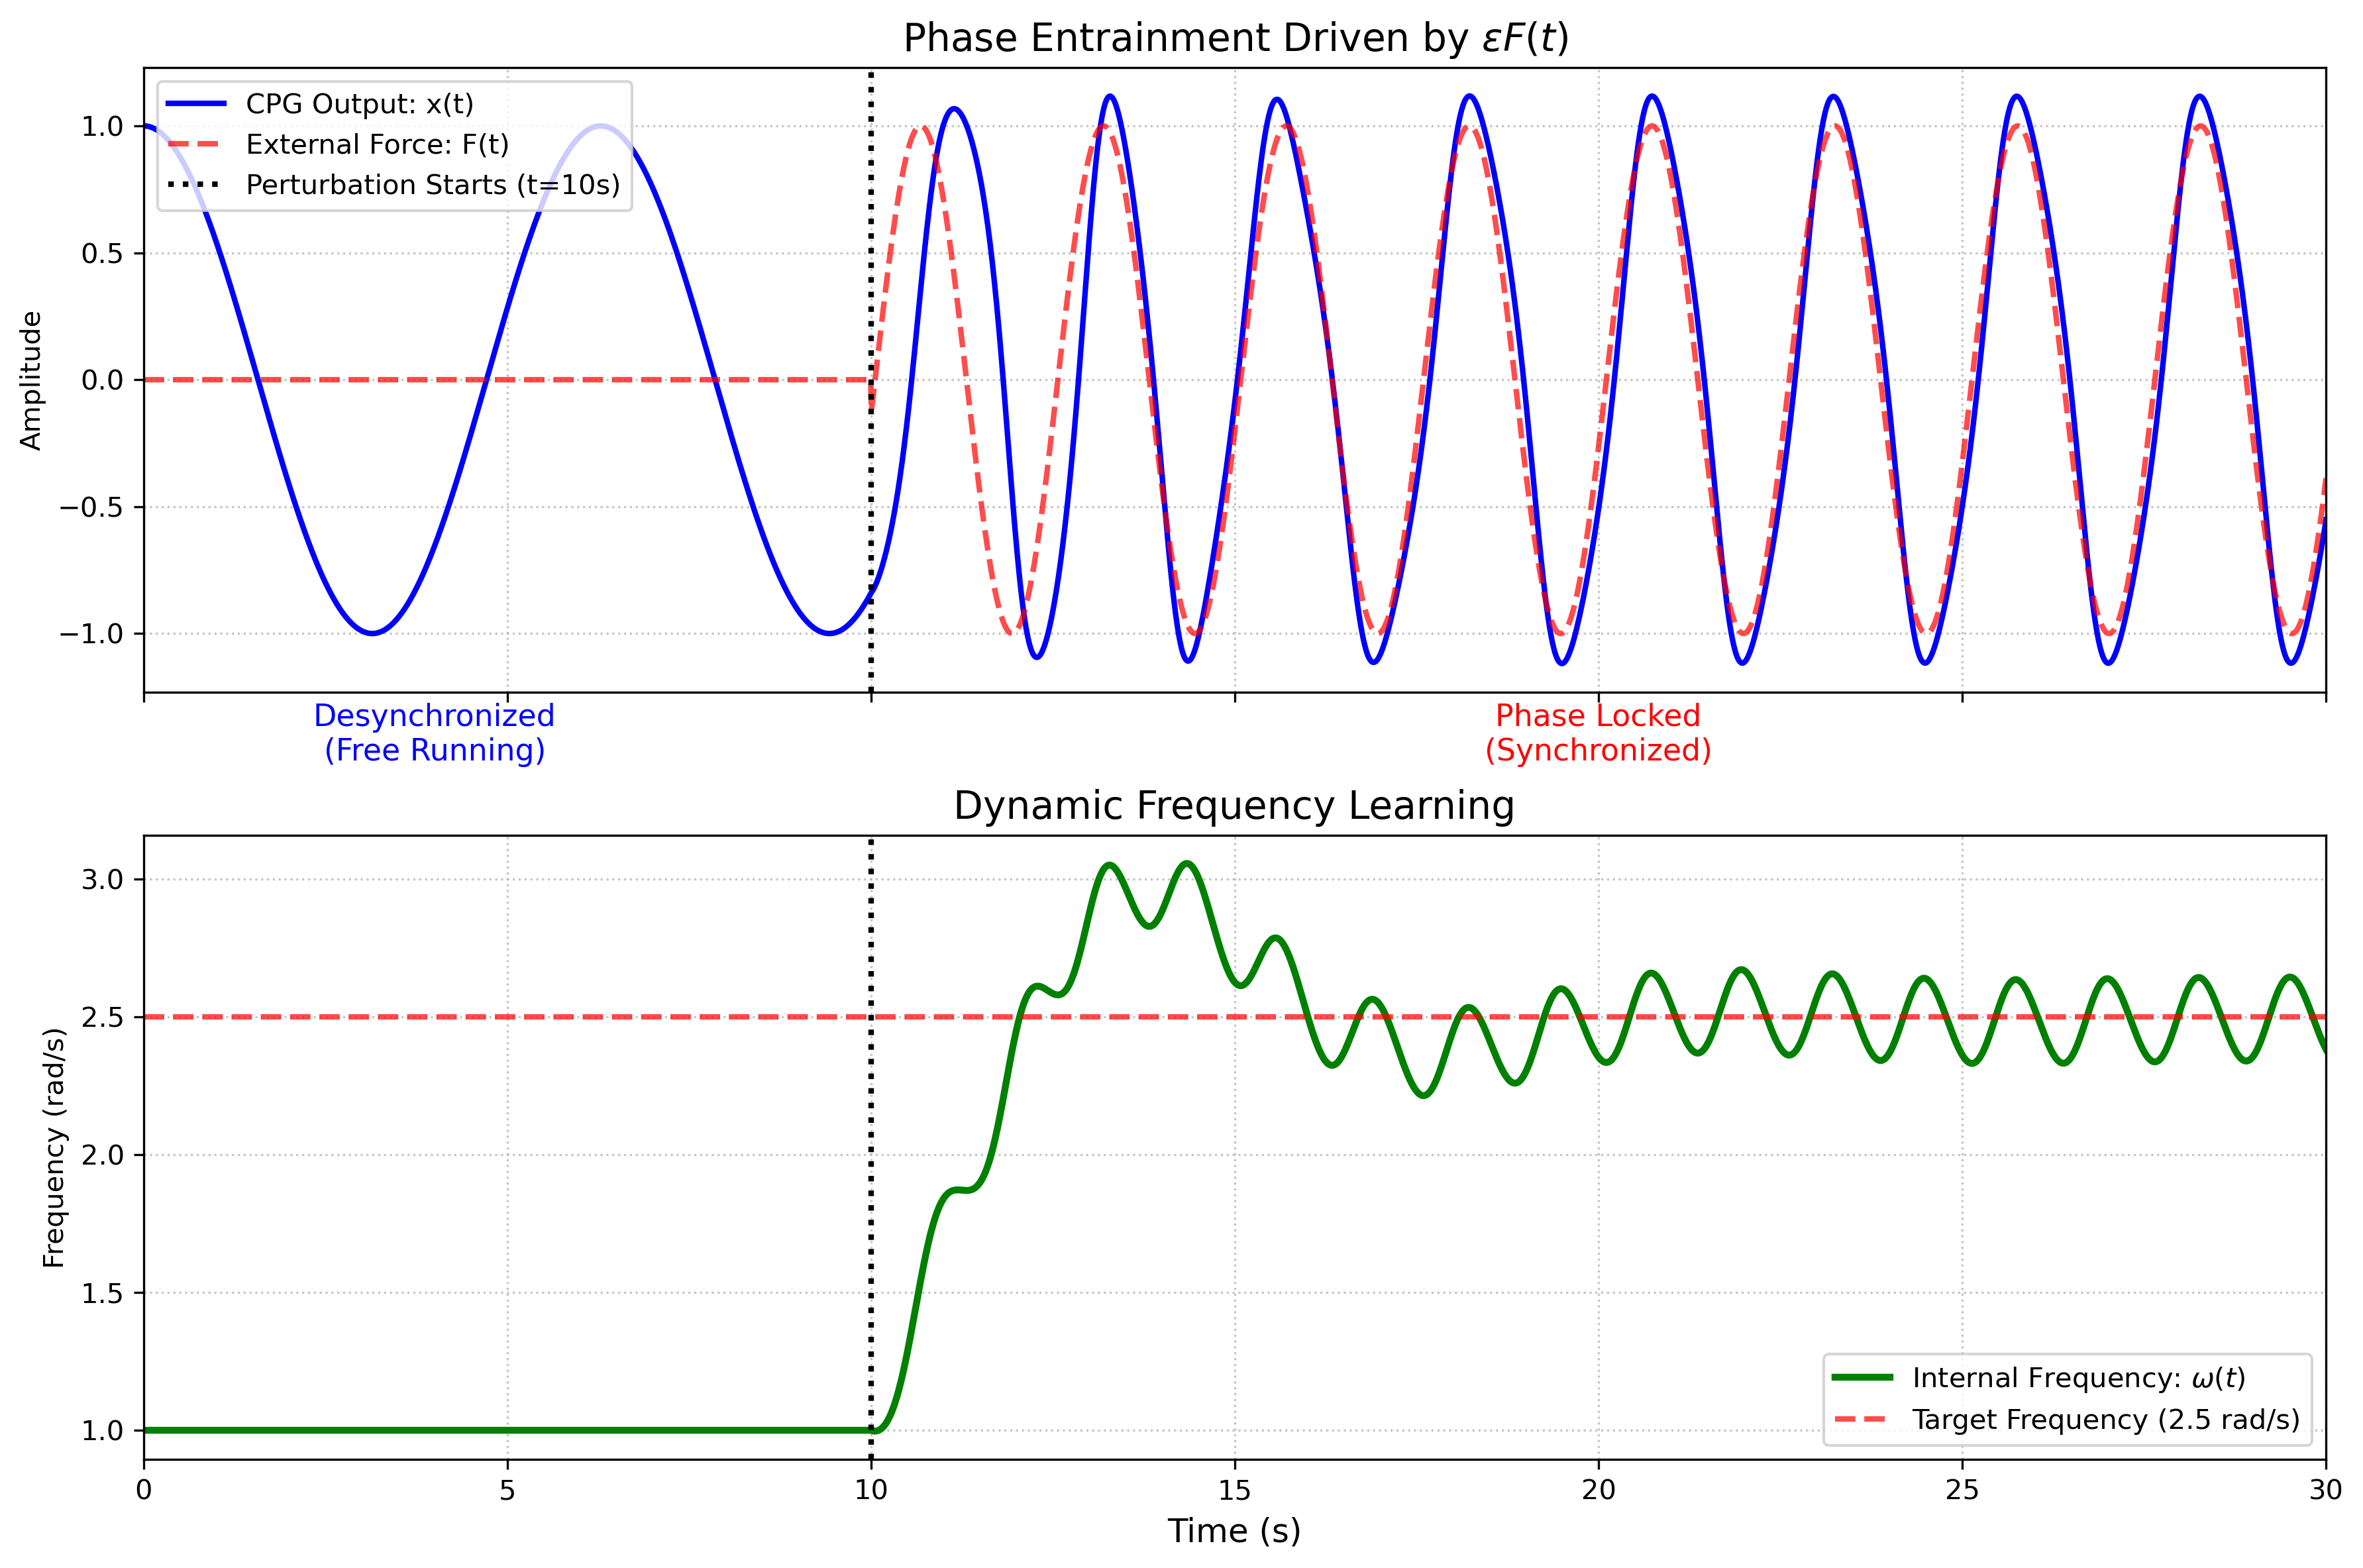
\includegraphics[width=0.95\textwidth]{figure/figure_source/figure2_entrainment.png} 
    \caption{耦合激励驱动下的系统相位同步与频率自适应演化过程}
    \label{fig:entrainment_mechanism}
\end{figure}

\section{耦合强度 $\varepsilon$ 对频率学习的影响推导}

在工程调参中，$\varepsilon$ 是决定学习性能的核心参数：它与\textbf{频率收敛速度呈正相关}，
但与\textbf{收敛后的稳态精度呈负相关} 。对此，我们可通过三角函数展开进行严格的理论证明 。
系统原来的表达式为：

\begin{equation}
    \begin{cases}
        \dot{x} = \gamma(\mu - r^2)x - \omega y + \varepsilon F(t) \\
        \dot{y} = \gamma(\mu - r^2)y + \omega x \\
        \dot{\omega} = -\varepsilon F(t) \frac{y}{r}
    \end{cases}
\end{equation}

假设系统已成功学习到外部频率并进入\textbf{锁相状态（Phase-locked state）}，此时

1. 外部连续扰动力可表示为：$F(t) = A \sin(\omega_{target} t)$
 
2. CPG 内部相位项可表示为：$\frac{y}{r} \approx \sin(\omega_{target} t + \phi)$，其中 $\phi$ 为稳态相位差 。

将上述稳态表达式代入频率学习方程 
\begin{equation}
    \dot{\omega} = -\varepsilon A \sin(\omega_{target} t) \sin(\omega_{target} t + \phi)
\end{equation}

利用积化和差公式 $\sin\alpha\sin\beta = \frac{1}{2}[\cos(\alpha-\beta) - \cos(\alpha+\beta)]$ 进行展开，得到 
\begin{equation}
    \dot{\omega} = -\frac{1}{2} \varepsilon A \cos(\phi) + \frac{1}{2} \varepsilon A \cos(2\omega_{target} t + \phi)
\end{equation}

\textbf{结论解析：}
\begin{itemize}
    \item \textbf{直流项} $-\frac{1}{2} \varepsilon A \cos(\phi)$：决定了系统的宏观稳态 。
    为保证 $\omega$ 整体不再漂移，必须满足 $\cos(\phi) = 0$，即内外信号严格锁定在特定相位差 。
    此时 $\phi = 90^\circ$ ，即$y$的相位为$\sin(\omega_{target} t + 90^\circ)$，也就是$\cos(\omega_{target} t)$。
    那么与它相差 $90^\circ$ 的输出变量 $x$，其相位自然就是 $\cos(\omega_{target} t - 90^\circ)$，也就是 $\sin(\omega_{target} t)$。
    此时 $x$ 的相位是 $\sin(\omega_{target} t)$，而外部力 $F(t)$ 也是 $A \sin(\omega_{target} t)$ 。
    即它们是完全同相的。
    \item \textbf{交流项} $+\frac{1}{2} \varepsilon A \cos(2\omega_{target} t + \phi)$：揭示了稳态波动的根源 。这是一个频率为 $2\omega_{target}$ 的高频波纹 。其振幅为 $\frac{1}{2} \varepsilon A$ 。
\end{itemize}

数学证明表明：稳态下 $\omega$ 必定在目标频率附近存在高频震荡，且\textbf{波动幅度与耦合强度 $\varepsilon$ 呈绝对的正比例关系} 。$\varepsilon$ 过大会导致输出轨迹携带高频噪声，严重时引发机械颤振或导致学习发散 。

% --- 预留插图位置 3 ---
\begin{figure}[htbp]
    \centering
    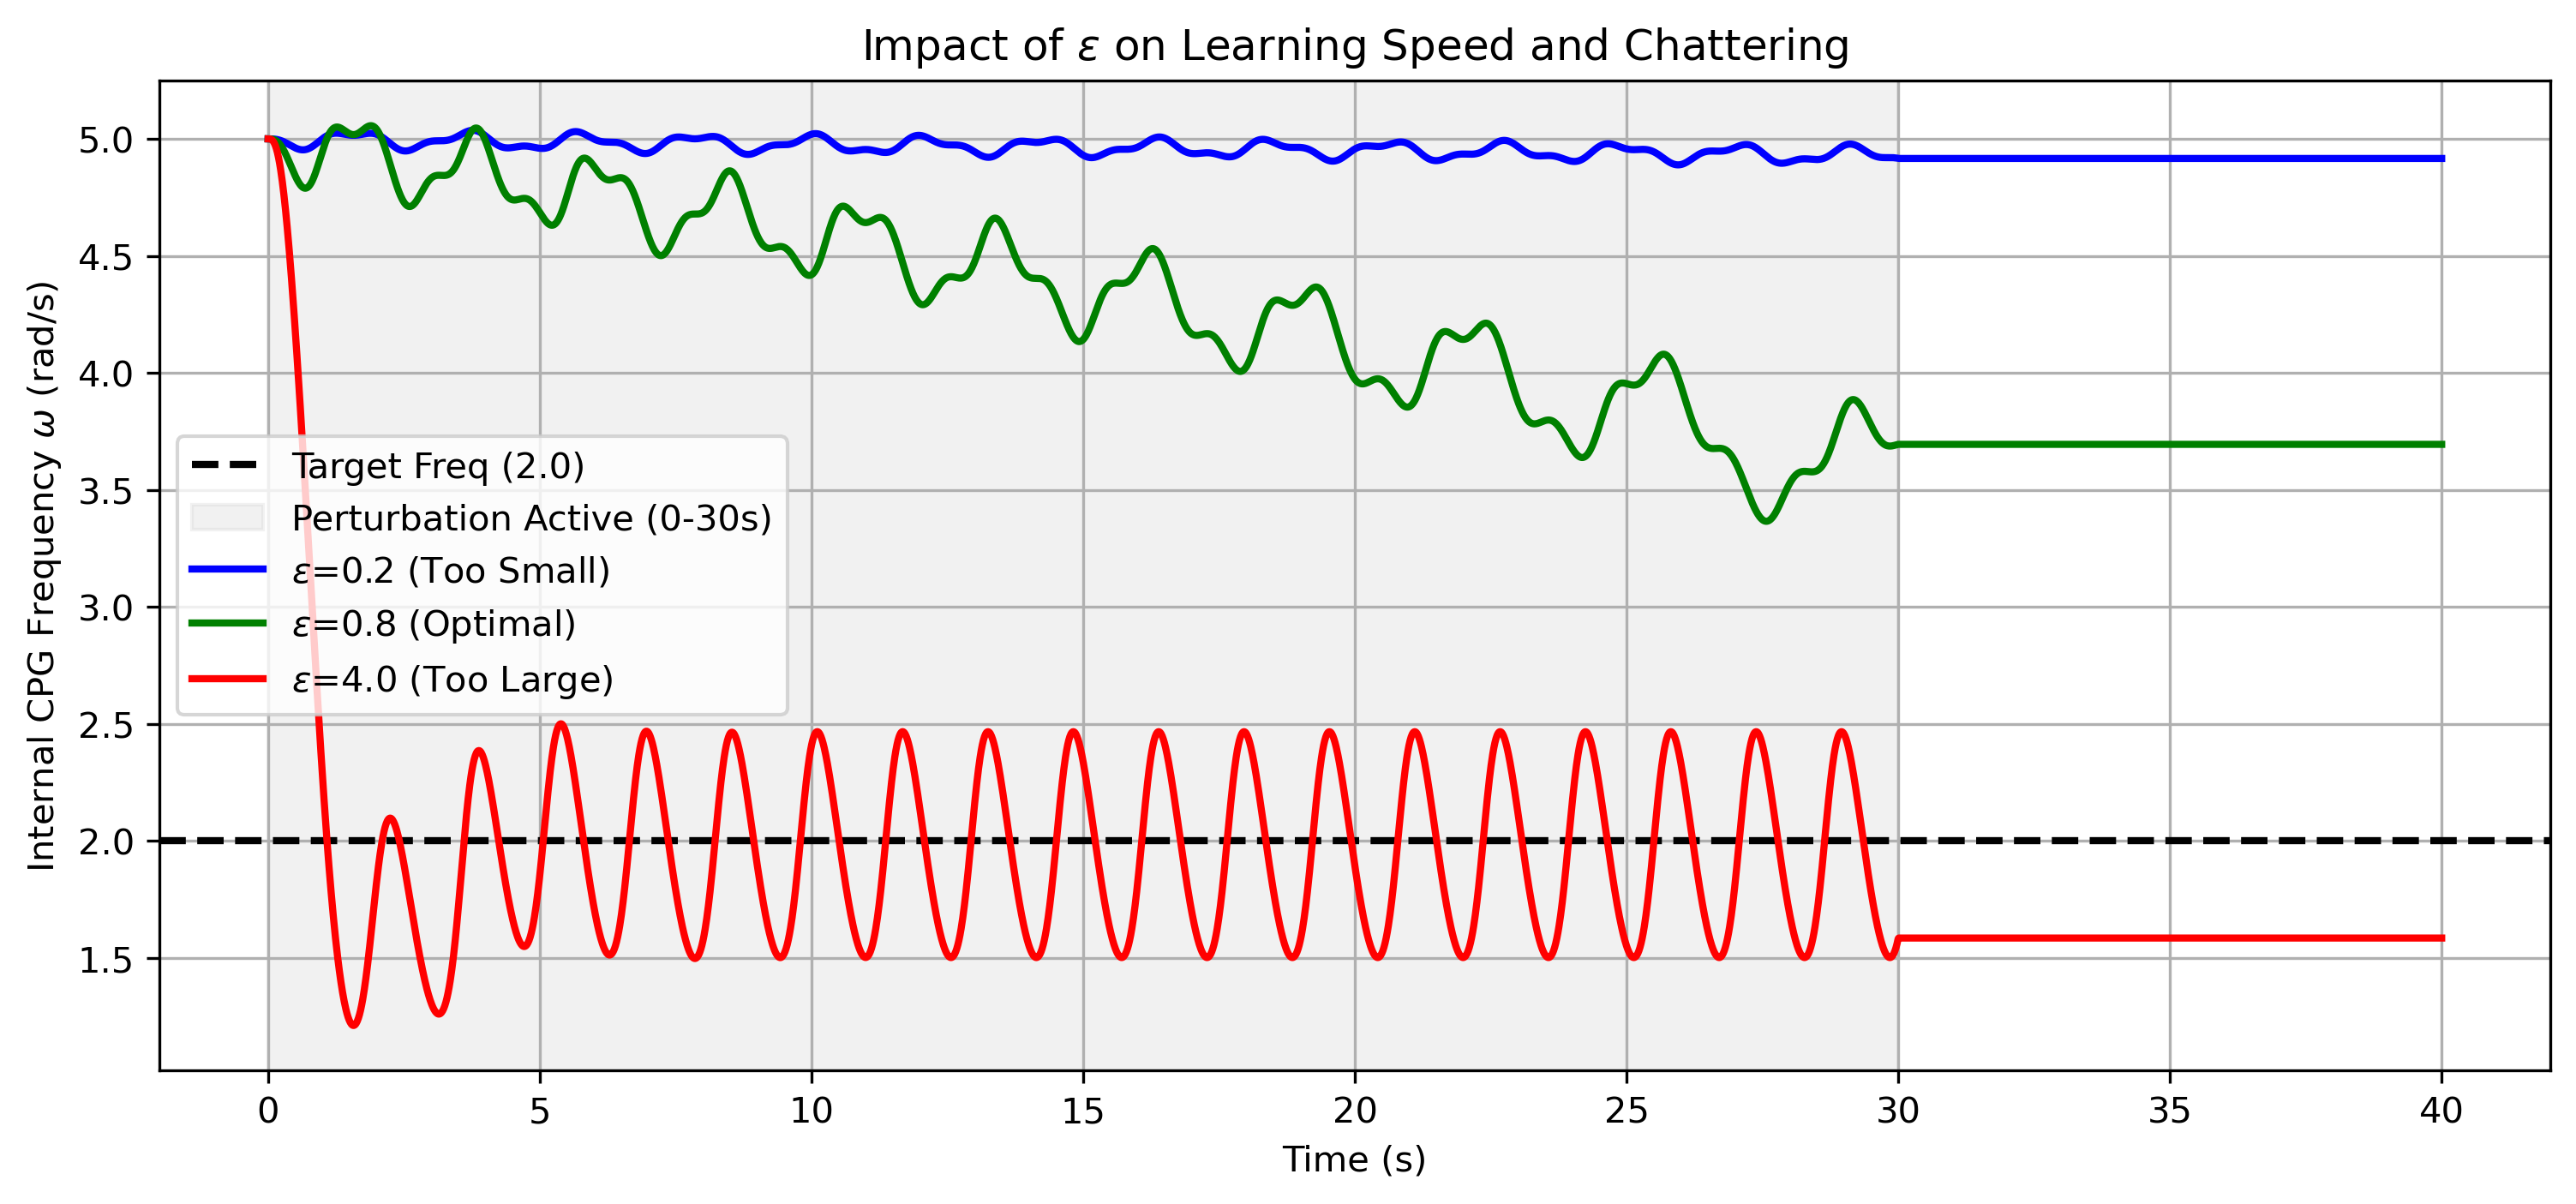
\includegraphics[width=0.8\textwidth]{figure/figure_source/figure3_epsilon_impact.png} 
    \caption{不同耦合强度 $\varepsilon$ 下内部频率 $\omega$ 的收敛速度与稳态震荡对比}
    \label{fig:epsilon_impact}
\end{figure}

\textbf{工程解决方案：低通滤波（LPF）的引入与权衡}

在实际的机器人底层控制部署中，上述理论推导指出了一个“死结”：为了让机器人快速适应突变的环境（要求极高的收敛速度），我们必须调大 $\varepsilon$；但这会直接导致稳态下控制信号出现不可接受的高频噪声和机械颤振 。

为了打破这一僵局，标准工程做法是在频率学习规则后串联一个\textbf{一阶低通滤波器}。
在代码实现中，我们将原方程积分得到的频率称为“原始学习频率” $\omega_{raw}$，而真正用于驱动 CPG 振荡器的则为“平滑频率” $\omega_{smooth}$，其动力学方程升级为：
\begin{equation}
    \tau \dot{\omega}_{smooth} + \omega_{smooth} = \omega_{raw}
\end{equation}
其中 $\tau$ 为滤波器的时间常数。

因此，低通滤波器能够极其精准地将这层“高频波纹”无情抹平，而完美保留代表真实学习结果的“直流项”。这意味着，我们可以放肆地调大 $\varepsilon$ 来追求极速自适应，同时保证最终输出的电机参考频率 $\omega_{smooth}$ 顺滑如丝。

\textbf{控制论的代价——相位延迟：}
然而，一切滤波皆有代价。增大时间常数 $\tau$ 虽然能获得极致的平滑度，但必然引入\textbf{相位延迟（Phase Delay）}。当外部环境频率发生二次突变时，过大的 $\tau$ 会导致机器人反应迟钝。因此，在实际 CPG 调参中，\textbf{学习率 $\varepsilon$（决定牵引力）与时间常数 $\tau$（决定平滑度与滞后）必须作为一对强耦合参数进行联合整定}，以达到灵敏度与稳定性的帕累托最优（Pareto Optimality）。

\begin{figure}[H]
    \centering
    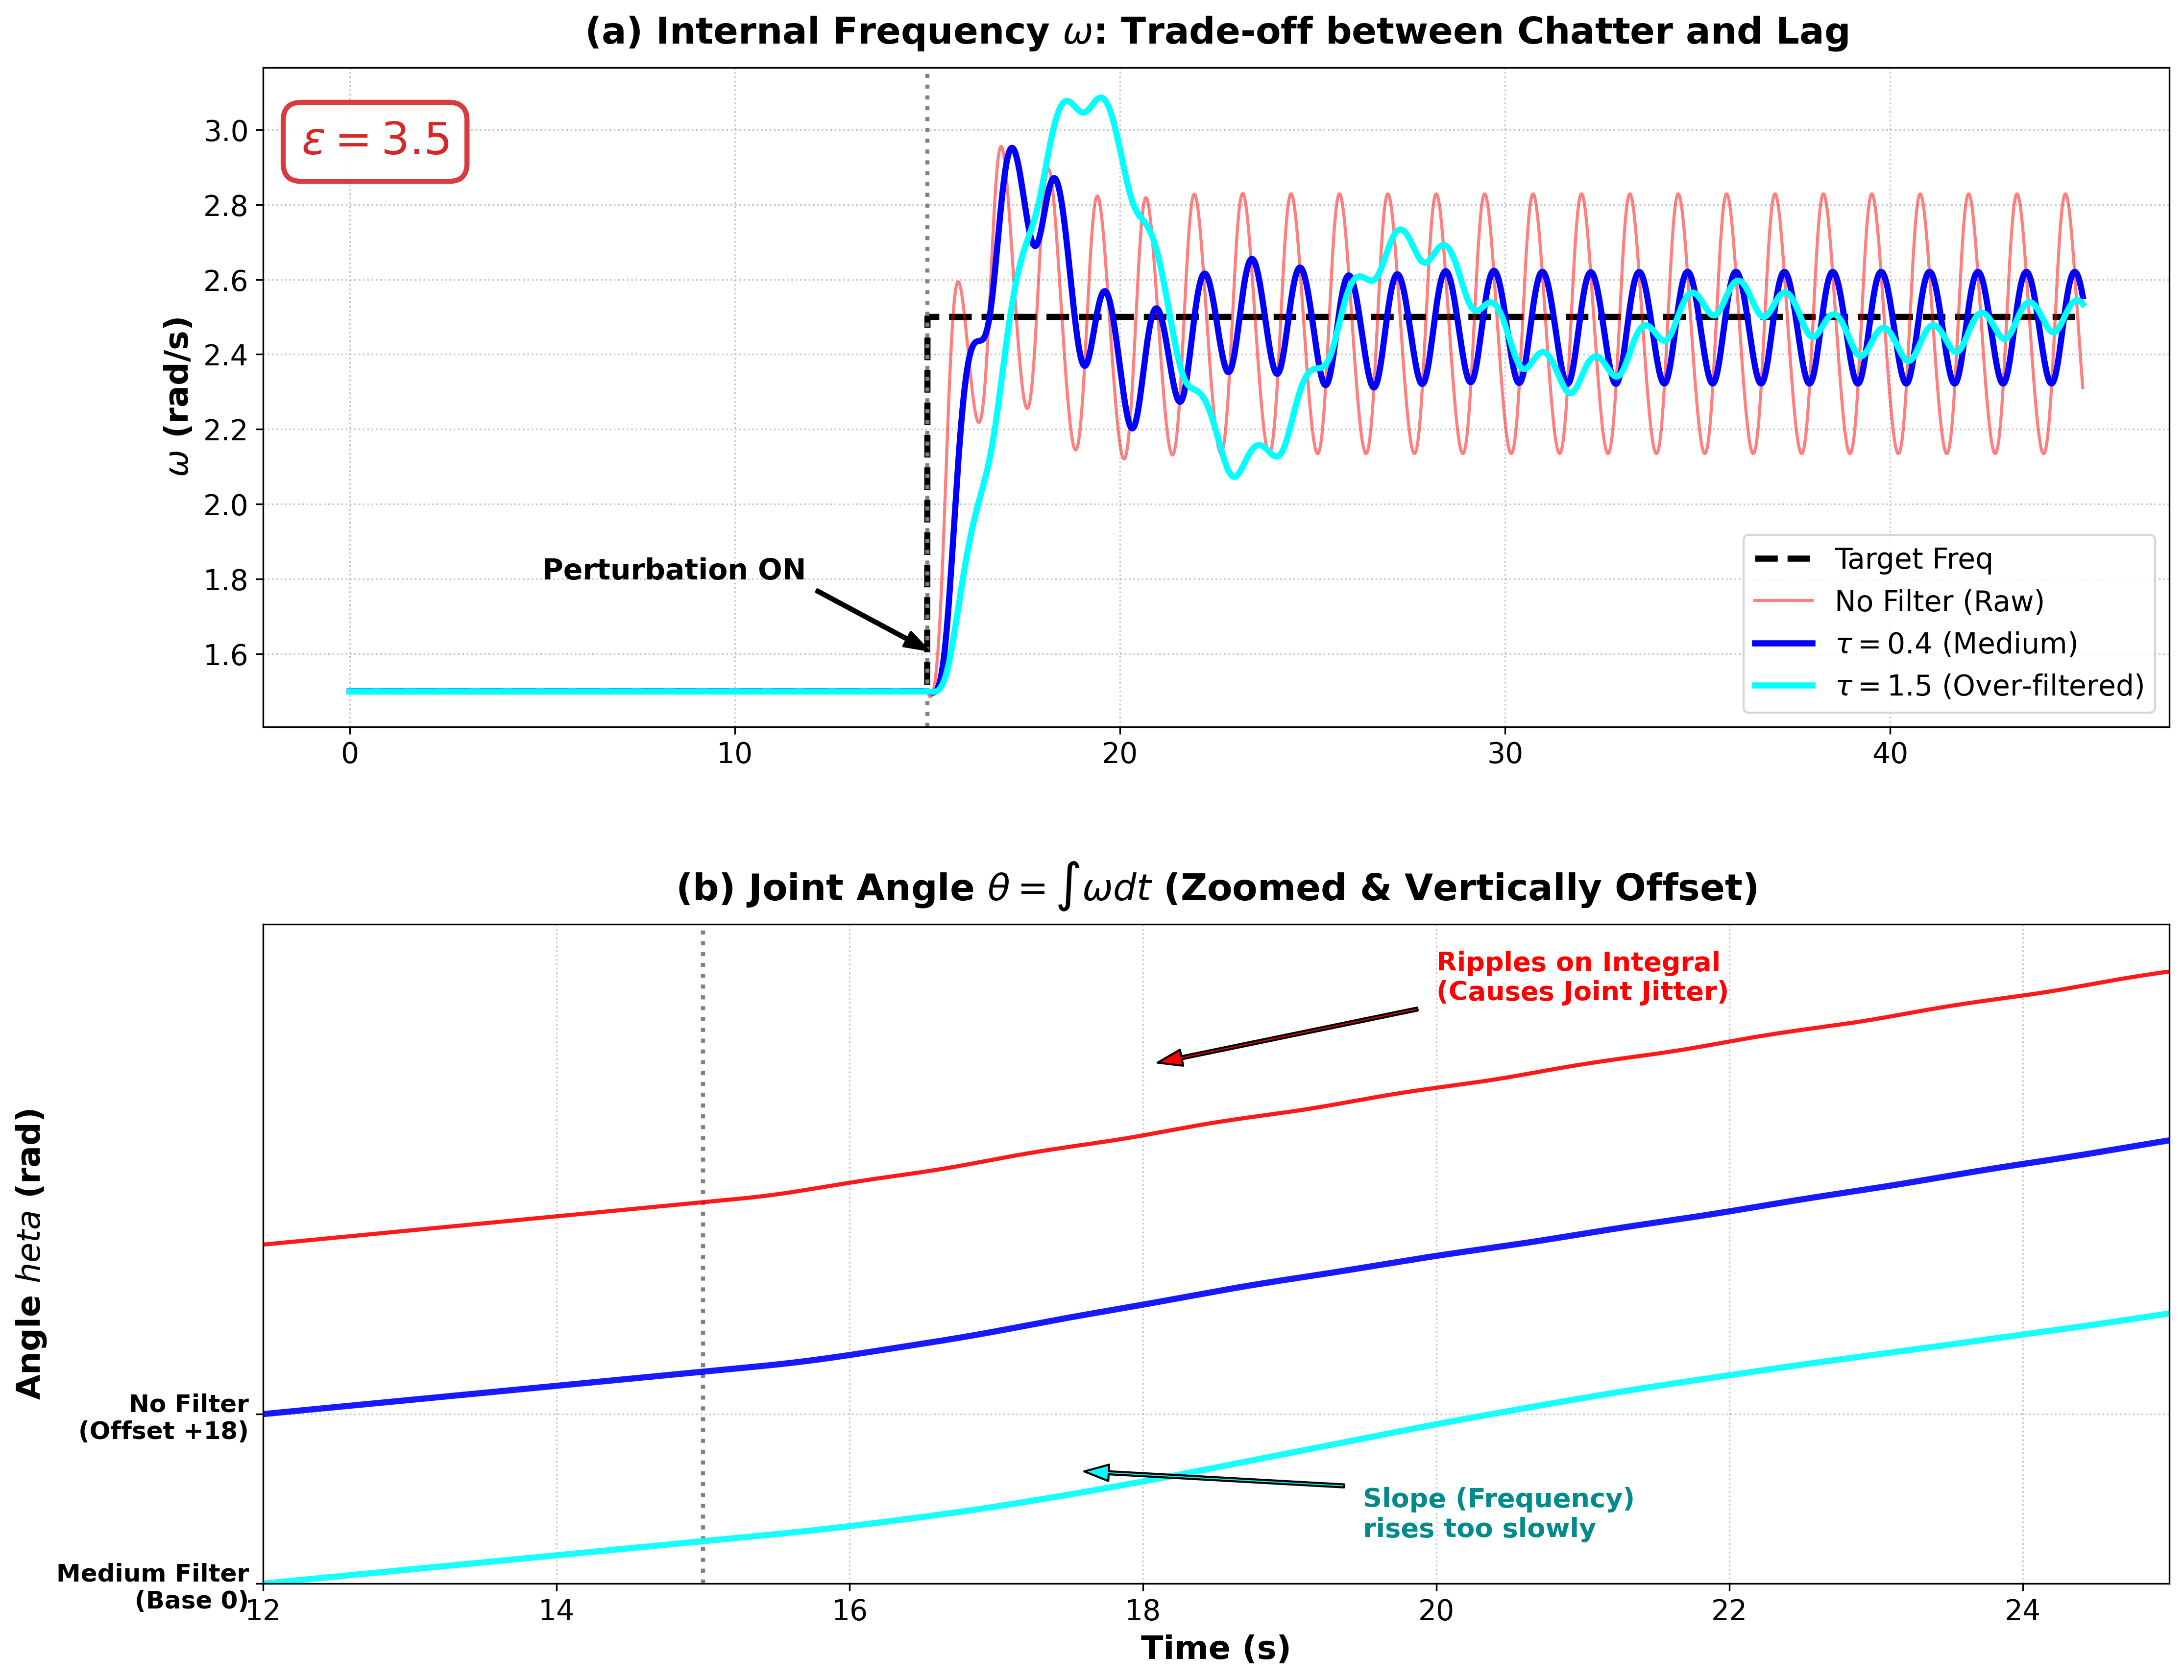
\includegraphics[width=1.0\textwidth]{figure/figure_source/figure_lpf_omega_vs_x.png} 
    \caption{不同滤波器情况对比}
    \label{fig:lfp_impact}
\end{figure}

\section{干扰信号频率 $\omega_{ext}$ 对频率学习 $\omega_{cpg}$ 的影响推导}
自适应 Hopf 振荡器的核心动力学方程如下：
$$\dot{x} = (\mu - x^2 - y^2)x - \omega y + \varepsilon F(t)$$
$$\dot{y} = (\mu - x^2 - y^2)y + \omega x$$
$$\dot{\omega} = -\varepsilon F(t) \frac{y}{\sqrt{x^2 + y^2}}$$
假设外部信号 $F(t) = A \sin(\phi_{ext})$，那么频率更新率 $\dot{\omega}$ 实际上正比于两个正弦信号的乘积：
$$\dot{\omega} \propto -\sin(\phi_{ext}) \sin(\phi_{cpg}) = \frac{1}{2} [\cos(\phi_{ext} + \phi_{cpg}) - \cos(\phi_{ext} - \phi_{cpg})]$$
当频率相近时（$\omega \approx \omega_{ext}$）：
相位差 $\phi_{ext} - \phi_{cpg}$ 变化得很慢，系统可以通过调整 $\omega$ 使得高频项被滤除，
低频项引导 $\omega$ 平稳收敛到 $\omega_{ext}$。
当频率相差悬殊时（比如 $\omega = 1, \omega_{ext} = 0.3$）：相位差 $\phi_{ext} - \phi_{cpg}$ 
随时间剧烈且快速地变化。此时，$\cos(\phi_{ext} - \phi_{cpg})$ 是一个高频振荡信号，
这意味着 $\dot{\omega}$ 在正负之间疯狂震荡。

\textbf{微积分补充：}假设有一个频率为 $\Omega$ 的余弦信号：$$\dot{\omega} = \cos(\Omega t)$$
$$\omega(t) = \int \cos(\Omega t) dt = \frac{1}{\Omega} \sin(\Omega t) + C$$

当 $\Omega$ 很小（低频信号，例如 $\Omega = 0.05$）：分母极小，放大倍数 $\frac{1}{\Omega} = 20$。
这意味着积分后的信号 $\omega(t) = 20 \sin(0.05 t)$。其振幅被剧烈放大，系统状态 $\omega$ 会产生巨大的偏移，
这个巨大的偏移引导系统去寻找新的平衡点，这就是“学习”的过程。

当 $\Omega$ 很大（高频信号，例如 $\Omega = 10$）：分母极大，衰减倍数 $\frac{1}{\Omega} = 0.1$。
这意味着积分后的信号 $\omega(t) = 0.1 \sin(10 t)$。其振幅被严重压缩，宏观上看，$\omega$ 的变化量只有区区 0.1，
它只能在初值附近做微小的抖动。高频信号在积分器面前“失效”了。

频率相近时（高频 + 低频）：
$$\dot{\omega} \propto \text{高频项}(\Omega_{sum}) + \text{低频项}(\Omega_{diff})$$
积分后：$$\omega(t) \propto \left( \frac{1}{\Omega_{sum}} \times \text{微小抖动} \right) + \left( \frac{1}{\Omega_{diff}} \times \text{巨大的宏观位移} \right)$$
高频项被积分器自动过滤（等于零），低频项接管了主导权，引导系统平稳收敛。

频率悬殊时（高频 + 高频）：
$$\dot{\omega} \propto \text{高频项}(\Omega_{sum}) + \text{相对高频项}(\Omega_{diff})$$积分后：$$\omega(t) \propto \left( \frac{1}{\text{大数}} \times \text{微小抖动} \right) + \left( \frac{1}{\text{较大数}} \times \text{微小抖动} \right)$$
两项的积分结果全是被压缩的微小震荡。系统中没有任何能够提供宏观位移的“低频牵引力”，
所以只能在原地发生毫无意义的紊乱（相位滑移），彻底丧失学习能力。

\begin{figure}[H]
    \centering
    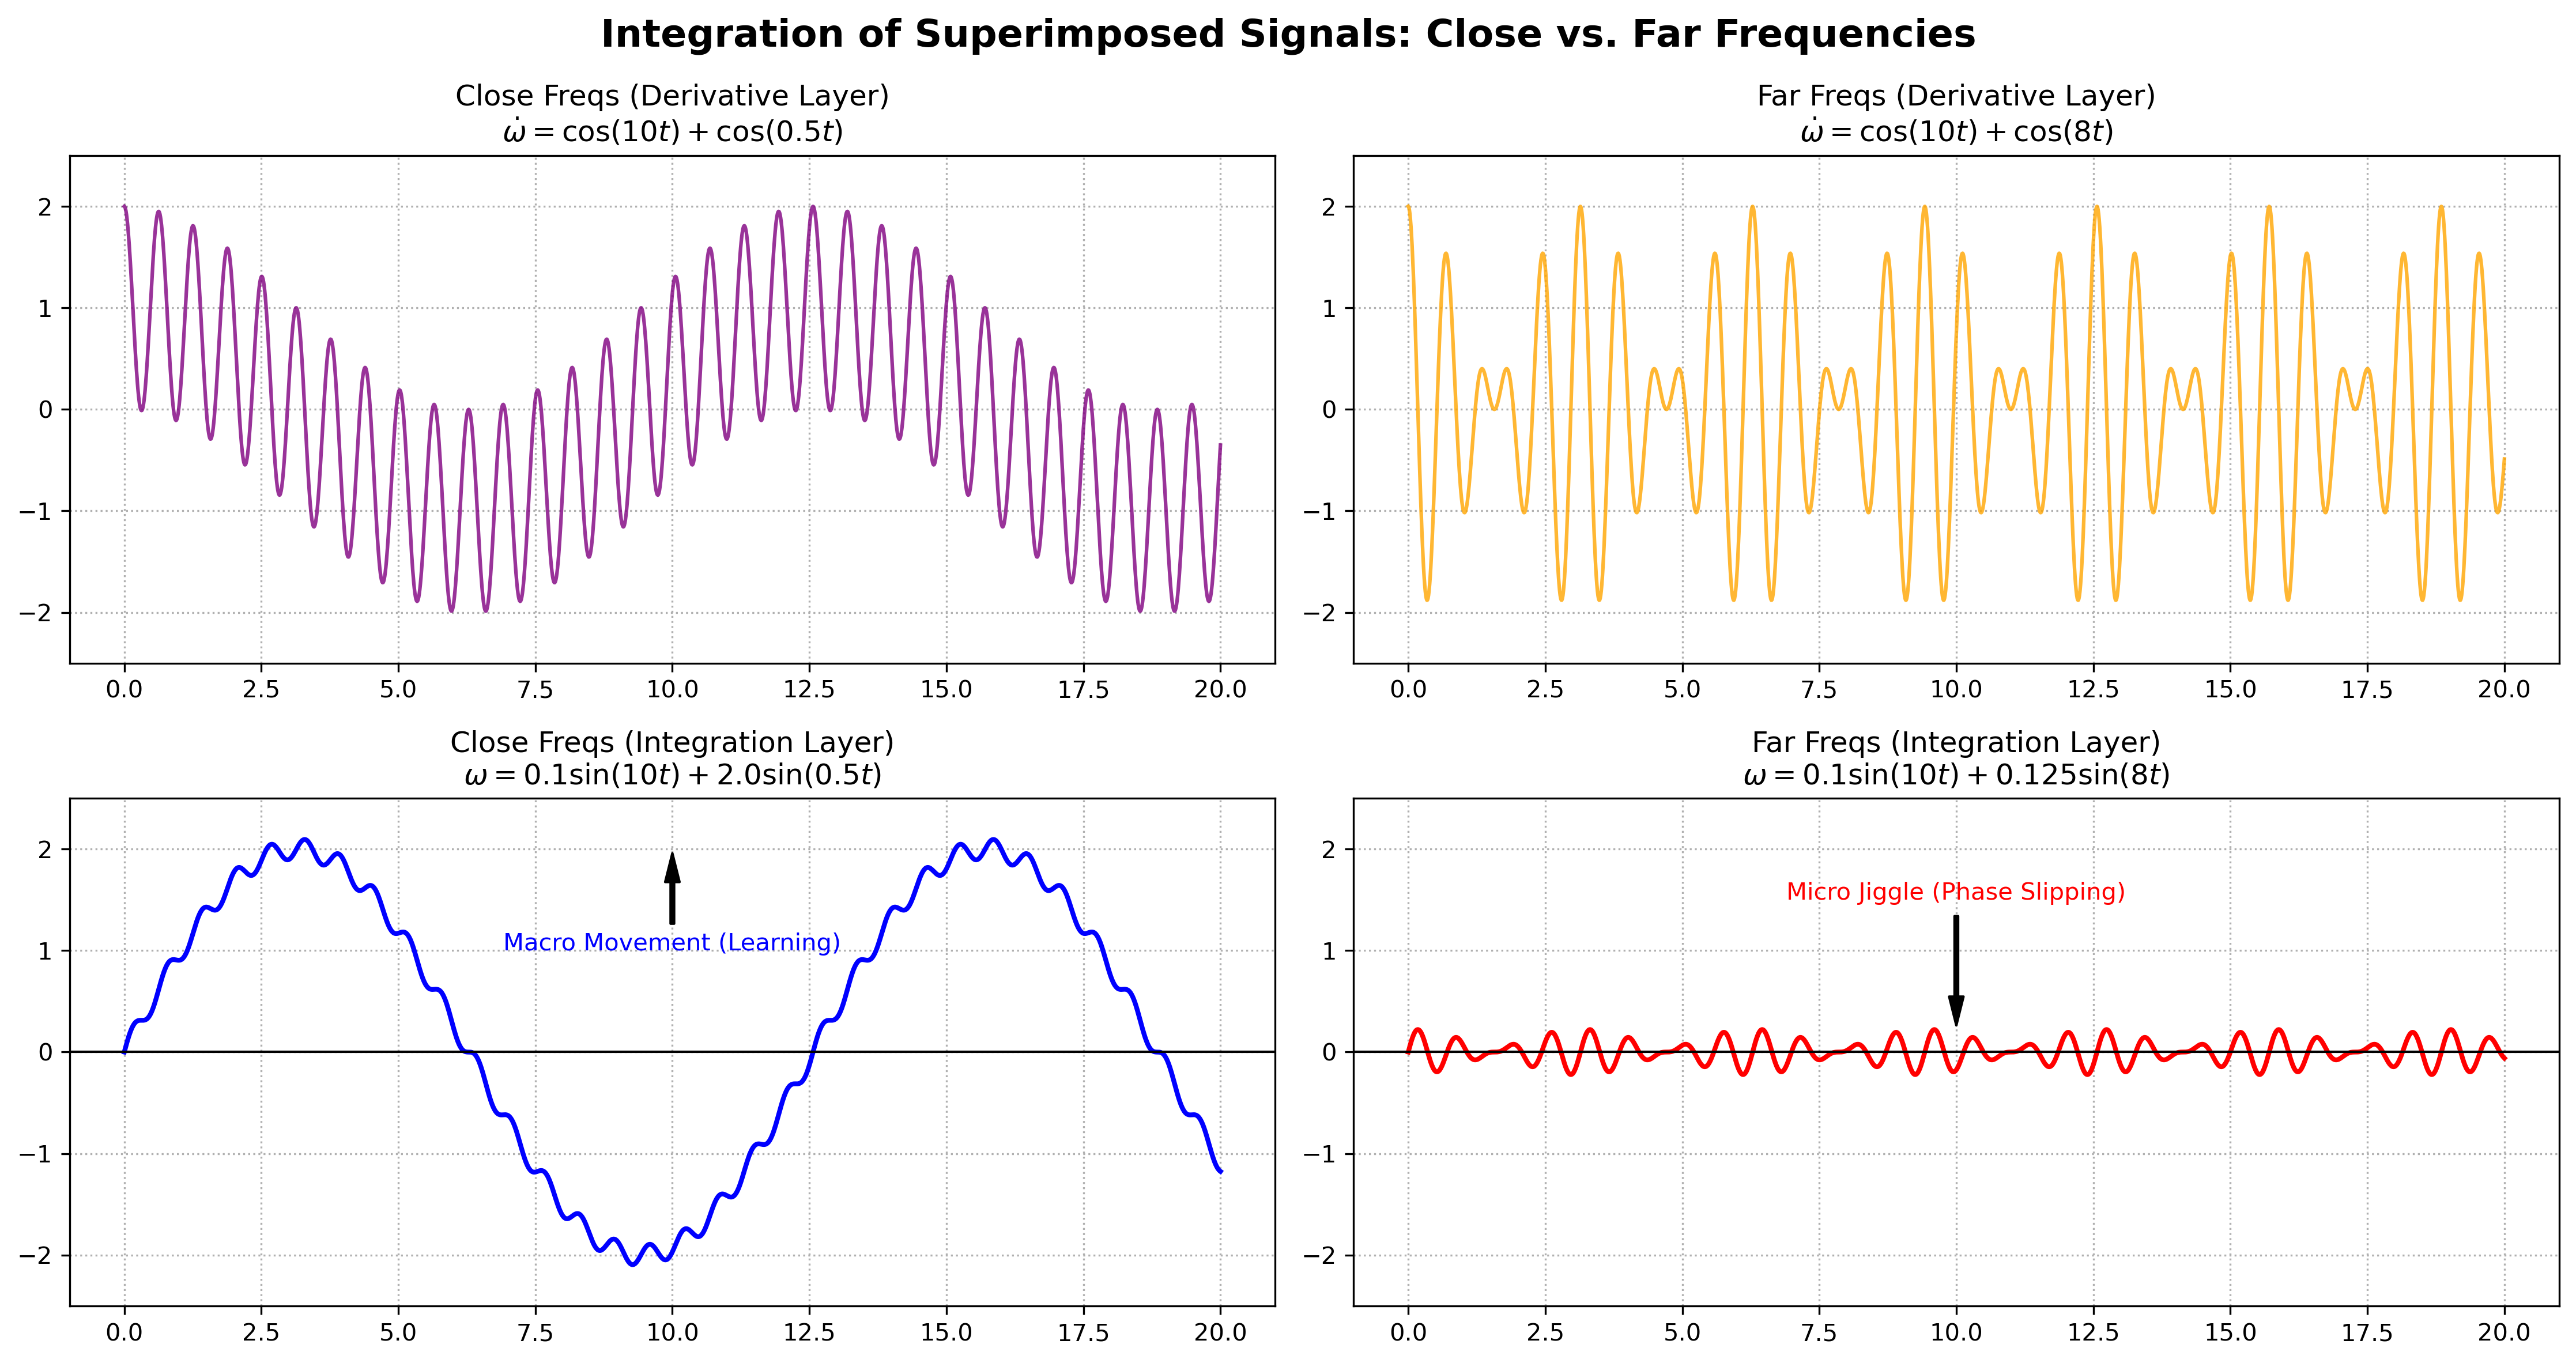
\includegraphics[width=1.0\textwidth]{figure/figure_source/figure4_integral_impact.png} 
    \caption{不同频率组合下频率 $\omega$ 积分情况对比}
    \label{fig:integral_impact}
\end{figure}

\textbf{真实CPG积分表达式推导:}真正的CPG频率学习微分方程是：
$$\dot{\omega} = -\varepsilon F(t) \sin(\phi_{cpg})$$
假设外部扰动 $F(t) = \sin(\omega_{ext} t)$，且在学习刚开始时，CPG的相位主要由其初始频率主导 
$\phi_{cpg} \approx \omega_{cpg} t$。
代入方程：$$\dot{\omega} = -\varepsilon \sin(\omega_{ext} t) \sin(\omega_{cpg} t)$$
根据三角函数积化和差公式 $\sin A \sin B = \frac{1}{2}[\cos(A-B) - \cos(A+B)]$，把负号放进去，得到真实的导数表达式：
$$\dot{\omega} = \frac{\varepsilon}{2} [ \cos((\omega_{ext} + \omega_{cpg})t) - \cos((\omega_{ext} - \omega_{cpg})t) ]$$
现在，对时间 $t$ 积分，得到真正的频率变化量 $\Delta \omega(t)$：
$$\Delta \omega(t) = \frac{\varepsilon}{2} \left[ \frac{1}{\omega_{ext} + \omega_{cpg}} \sin((\omega_{ext} + \omega_{cpg})t) - \frac{1}{\omega_{ext} - \omega_{cpg}} \sin((\omega_{ext} - \omega_{cpg})t) \right]$$

当$\omega_{cpg}$和$\omega_{ext}$相近时：
相位差 $\phi_{ext} - \phi_{cpg}$ 变化很慢且接近于0,其差频项倒数数值较大，占据主导地位，
$\Delta \omega(t)$处于大振幅低频率状态，即学习状态。


当$\omega_{cpg}$和$\omega_{ext}$差距过大时：
相位差 $\phi_{ext} - \phi_{cpg}$ 与相位和 $\phi_{ext} + \phi_{cpg}$ 均处于较大状态，
$\Delta \omega(t)$整体处于高频率小振幅状态，即相位漂移状态。

\textbf{结论解析:}相差过大导致相位滑移（Phase Slipping）。$\omega$ 的导数变成了宽频噪声的积分，
$\omega$ 只能在原地剧烈抖动，或者因为非线性系统的局部极小值（Spurious Attractors）而发生不可逆的漂移。
一旦扰动撤去，$\omega$ 已经漂移到了一个错误的、使得系统能量达到某种局部平衡的低频区域，再也回不去了。

\begin{figure}[H]
    \centering
    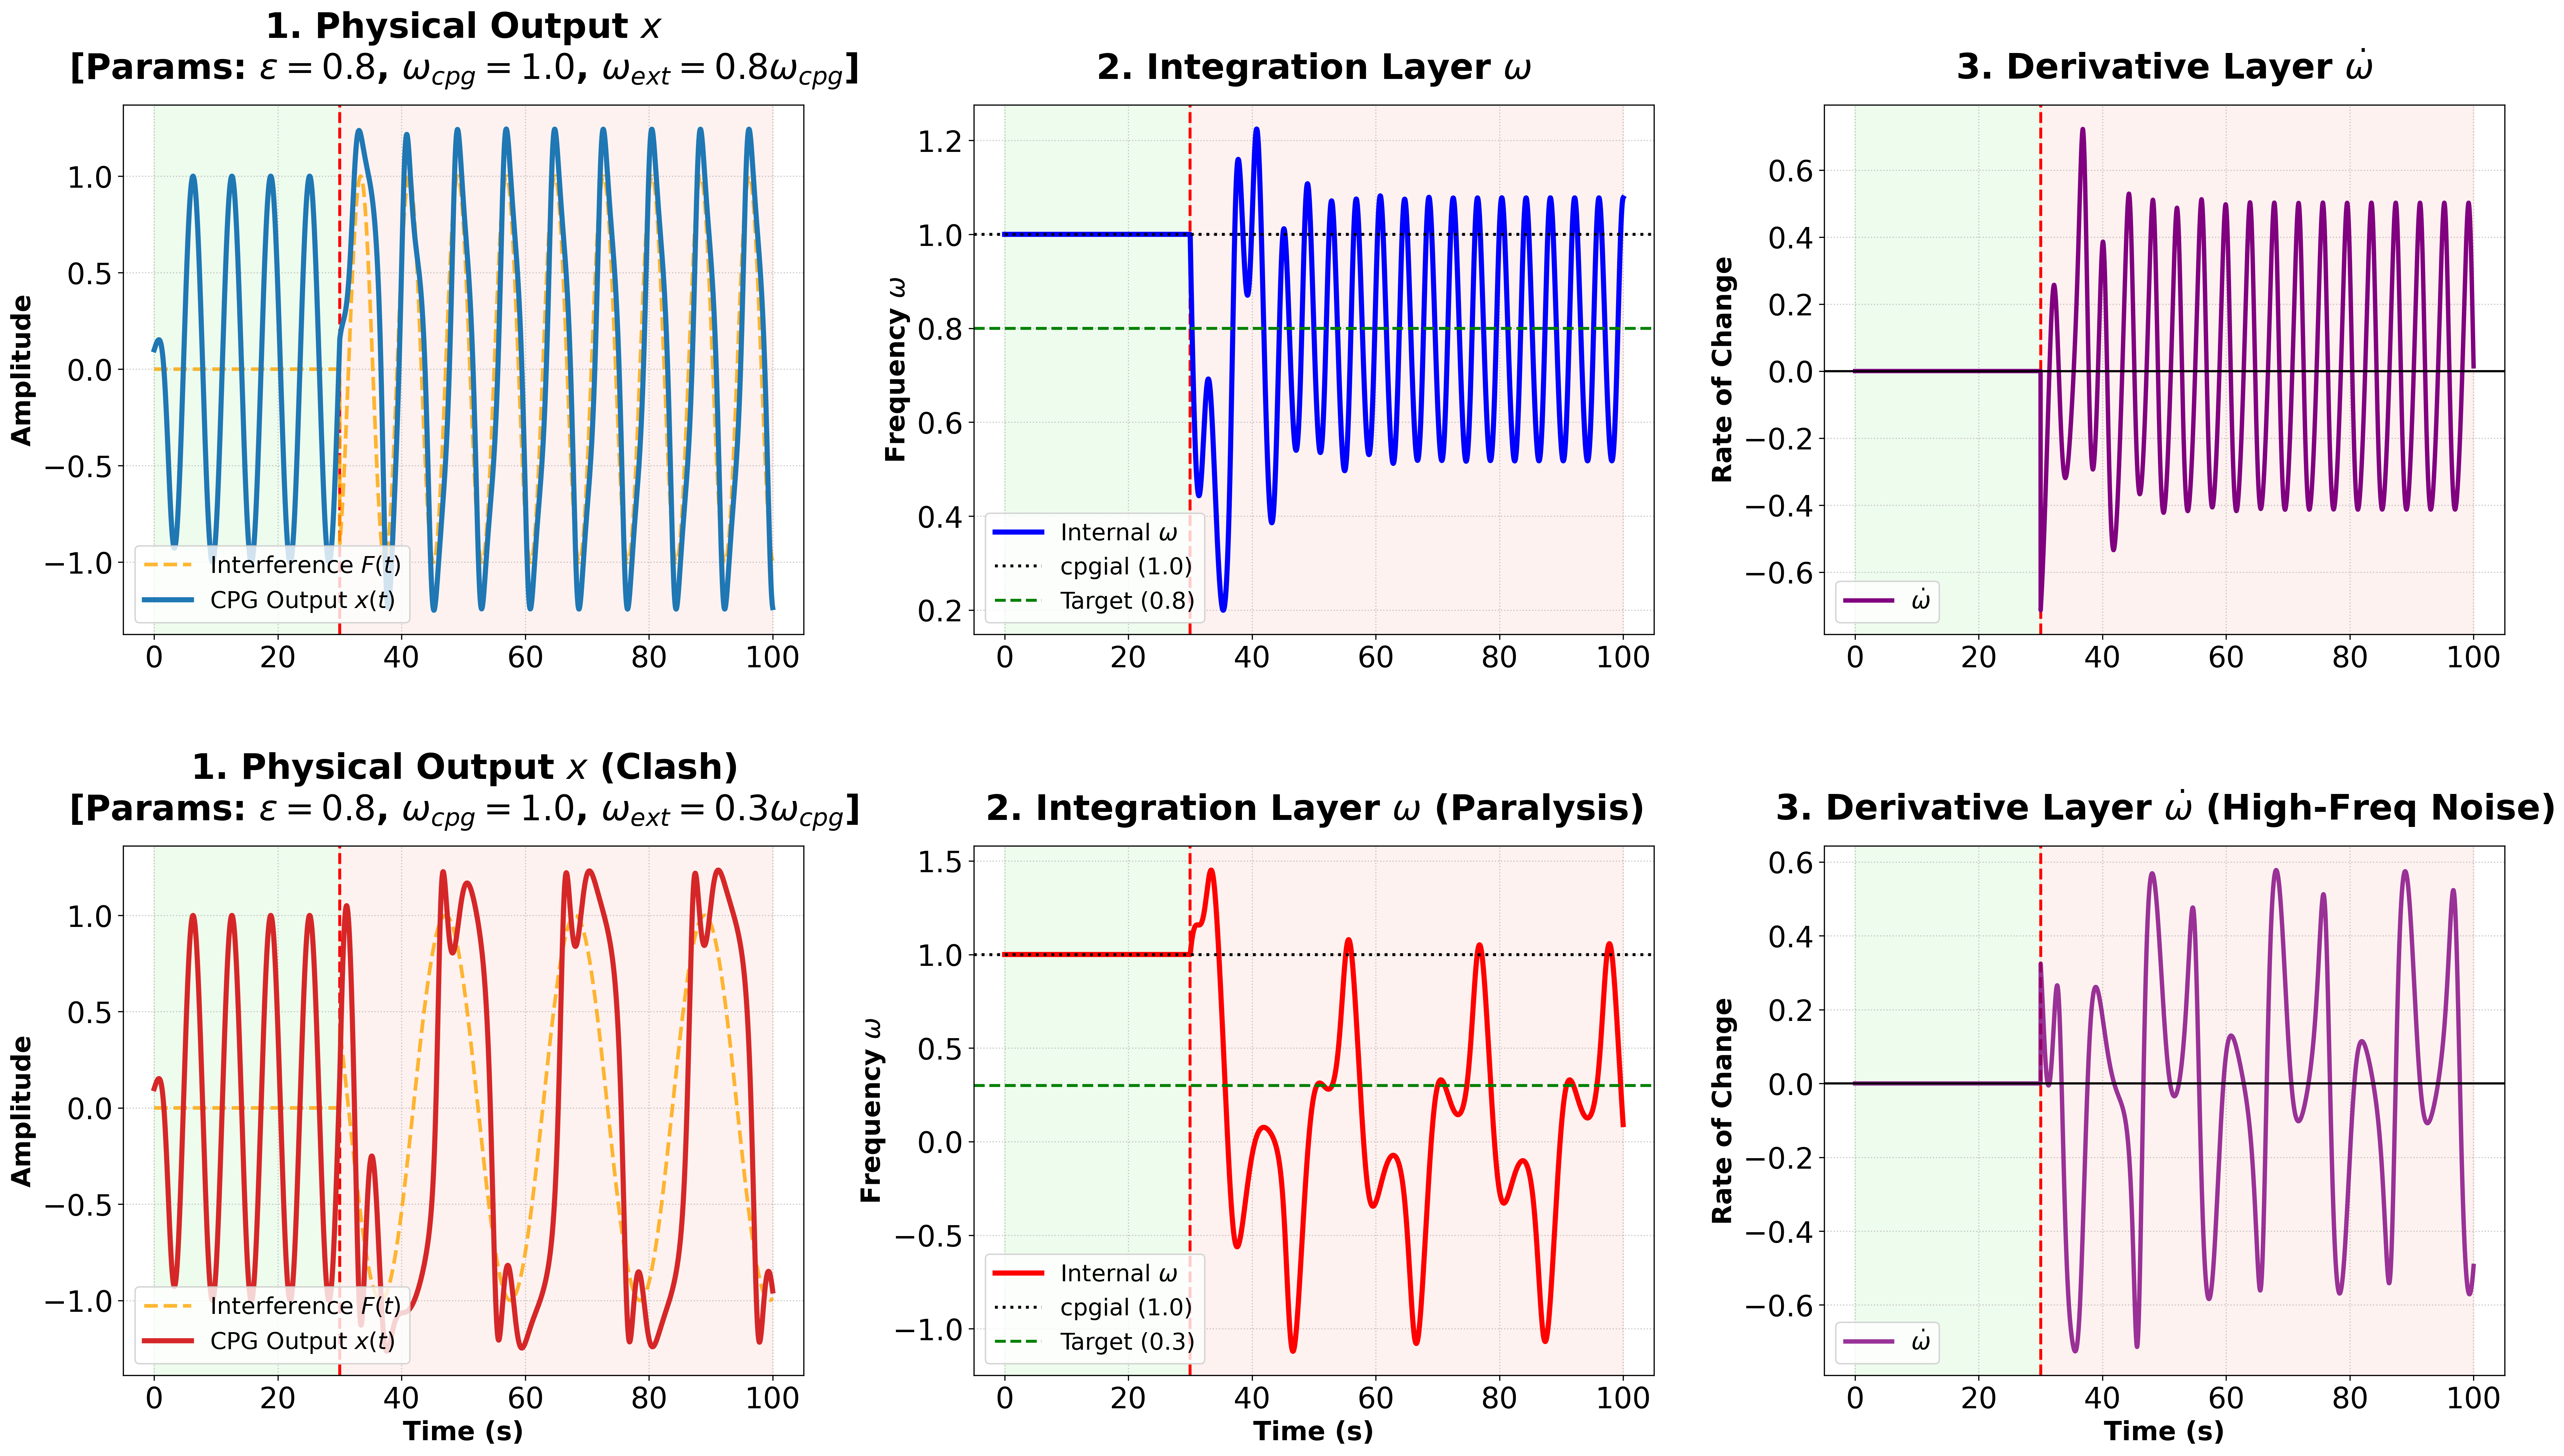
\includegraphics[width=1.0\textwidth]{figure/figure_source/cpg_full_pipeline.png} 
    \caption{不同干扰信号频率 $\omega_{ext}$ 下内部频率 $\omega_{cpg}$ 的收敛速度与稳态震荡展示}
    \label{fig:omega_ext_impact}
\end{figure}

\section{多干扰信号对频率学习的影响推导}

将自适应 Hopf 振荡器的动力学方程从笛卡尔坐标系 $(x, y)$ 转换到极坐标系 $(r, \phi)$。设状态变量为：$$x = r \cos\phi$$$$y = r \sin\phi$$其中，$r$ 是瞬时振幅，$\phi$ 是瞬时相位。将这组变换代入我们之前的 Hopf 频率更新方程中：$$\dot{\omega} = -\varepsilon F(t) \frac{y}{\sqrt{x^2 + y^2}}$$因为 $\sqrt{x^2 + y^2} = r$，方程可以极大地化简为：$$\dot{\omega} = -\varepsilon F(t) \sin\phi$$这说明：内部频率的演化 $\dot{\omega}$，本质上取决于外部输入 $F(t)$ 与CPG当前状态 $\sin\phi$ 的乘积。

现在，把含有两个频率分量的复合信号输入CPG模型：$$F(t) = A_1 \sin(\omega_1 t) + A_2 \sin(\omega_2 t)$$将其代入 $\dot{\omega}$ 的方程中：$$\dot{\omega} = -\varepsilon [A_1 \sin(\omega_1 t) + A_2 \sin(\omega_2 t)] \sin\phi$$利用三角函数积化和差公式 $\sin\alpha \sin\beta = \frac{1}{2}[\cos(\alpha - \beta) - \cos(\alpha + \beta)]$，将方程展开：$$\dot{\omega} = \frac{\varepsilon A_1}{2} [\cos(\omega_1 t + \phi) - \cos(\omega_1 t - \phi)] + \frac{\varepsilon A_2}{2} [\cos(\omega_2 t + \phi) - \cos(\omega_2 t - \phi)]$$

假设CPG当前的内部频率 $\omega$ 接近于输入信号的第一个频率 $\omega_1$（或者在初始状态下靠得比较近）。那么，CPG 的相位 $\phi$ 可以近似表示为 $\phi(t) \approx \omega_1 t + \psi_1$，其中 $\psi_1$ 是相位差。我们将方程中的四个余弦项进行分类：

高频振荡项（快变量）：$$\cos(\omega_1 t + \phi) \approx \cos(2\omega_1 t + \psi_1)$$$$\cos(\omega_2 t + \phi) \approx \cos((\omega_1 + \omega_2)t + \psi_1)$$$$\cos(\omega_2 t - \phi) \approx \cos((\omega_2 - \omega_1)t - \psi_1)$$
由于这些项都含有关于时间 $t$ 的高频变化成分，根据积分平均化理论，在一个较长的时间窗口内，这些高频项的积分平均值趋近于0。它们只会在 $\omega$ 附近引起微小的“高频抖动”，不会产生长期的漂移趋势。

低频慢漂移项（慢变量）：观察 $-\cos(\omega_1 t - \phi)$ 这一项。因为 $\phi \approx \omega_1 t + \psi_1$，所以 $\omega_1 t - \phi \approx -\psi_1$。这一项变成了 $-\cos(-\psi_1) = -\cos\psi_1$。注意，$\psi_1$ 相对于时间 $t$ 是一个变化非常缓慢的量（因为 $\dot{\phi}$ 和 $\omega_1$ 极其接近）。

经过平均化滤波（Averaging Filter）后，高频项全部被抹平，系统关于频率更新的宏观动力学方程坍缩为：$$\langle \dot{\omega} \rangle \approx -\frac{\varepsilon A_1}{2} \cos\psi_1$$

当 $\omega$ 靠近 $\omega_1$ 时，输入信号中 $\omega_2$ 所产生的所有动态项 $\cos(\omega_2 t \pm \phi)$ 都变成了快变量，被动力学系统的积分特性像“低通滤波器”一样直接滤除了（即不产生长期的 $\dot{\omega}$ 驱动力）。系统最终只剩下由 $\omega_1$ 驱动的慢变量动态 $\langle \dot{\omega} \rangle \approx -\frac{\varepsilon A_1}{2} \cos\psi_1$。这个方程会持续调整 $\omega$，直到系统满足稳态锁相条件（Phase Locking Condition）：当 $\langle \dot{\omega} \rangle = 0$ 时，必须有 $\cos\psi_1 = 0$。这意味着最终 $\psi_1 = \pm \frac{\pi}{2}$，即 CPG 的输出与输入信号 $\omega_1$ 保持严格的 $\mathbf{90^\circ}$ 相位差，此时 CPG 的内部频率 $\omega$ 完全且永久地收敛到了 $\omega_1$。

\vspace{10pt}
\textbf{$90^\circ$ 相位差补充：}在实际动力学稳定域中，它会收敛到 $\psi_1 = -\frac{\pi}{2}$。

在非线性动力学中，方程的根（平衡点）有很多个，但并非所有的平衡点都能在物理世界中存在。要证明系统为什么一定会收敛到 $\psi_1 = -\frac{\pi}{2}$ 而不是 $+\frac{\pi}{2}$，需使用：局部线性化与雅可比矩阵（Jacobian Matrix）的稳定性分析。

在前一次推导中，我们只看了频率的演化$\dot{\omega}$。为了分析稳定性，我们必须同时看相位差的演化 $\dot{\psi}_1$，它们构成了一个相互耦合的二维动力学系统。首先，回到最初的笛卡尔极坐标系。我们知道 CPG 的状态方程是：
$$\dot{x} = \gamma (\mu - r^2)x - \omega y + \varepsilon F(t)$$$$\dot{y} = \gamma (\mu - r^2)y + \omega x$$通过坐标变换 $x = r \cos\phi, y = r \sin\phi$，可以推导出瞬时相位 $\phi$ 的微分方程（过程省略，利用 $\tan\phi = y/x$ 求导可得）：$$\dot{\phi} = \omega - \frac{\varepsilon}{r} F(t) \sin\phi$$

现在，定义两个变量来描述系统向目标状态逼近的过程：

频率误差：$\Delta\omega = \omega - \omega_1$

相位差：$\psi_1 = \phi - \omega_1 t$

对这两个慢变量求导，并代入外部输入 $F(t) = A_1 \sin(\omega_1 t)$，再根据前文的平均化理论滤除高频项，就得到了这个二维耦合系统的宏观演化方程：频率误差动力学：$$\dot{\Delta\omega} = \langle \dot{\omega} \rangle = -\frac{\varepsilon A_1}{2} \cos\psi_1$$相位差动力学（注意 $\dot{\psi}_1 = \dot{\phi} - \omega_1$）：$$\dot{\psi}_1 = \Delta\omega - \frac{\varepsilon A_1}{2r} \cos\psi_1$$

系统达到稳态（平衡点）的数学定义是：状态变量不再随时间变化，即导数为 0。
令 $\dot{\Delta\omega} = 0$ 且 $\dot{\psi}_1 = 0$：$$-\frac{\varepsilon A_1}{2} \cos\psi_1 = 0 \implies \cos\psi_1 = 0 \implies \psi_1^* = \pm \frac{\pi}{2}$$将 $\cos\psi_1 = 0$ 代入第二个方程得：$$\Delta\omega - 0 = 0 \implies \Delta\omega^* = 0 \implies \omega^* = \omega_1$$所以，数学上确实存在两个平衡点：$(0, +\frac{\pi}{2})$ 和 $(0, -\frac{\pi}{2})$。

雅可比矩阵与特征值分析 (Stability Analysis):

在平衡点处对非线性方程组进行泰勒展开，求其一阶偏导数组成的雅可比矩阵 $J$：$$J = \begin{bmatrix} \frac{\partial \dot{\Delta\omega}}{\partial \Delta\omega} & \frac{\partial \dot{\Delta\omega}}{\partial \psi_1} \\ \frac{\partial \dot{\psi}_1}{\partial \Delta\omega} & \frac{\partial \dot{\psi}_1}{\partial \psi_1} \end{bmatrix} = \begin{bmatrix} 0 & \frac{\varepsilon A_1}{2} \sin\psi_1 \\ 1 & \frac{\varepsilon A_1}{2r} \sin\psi_1 \end{bmatrix}$$
根据线性系统控制理论，一个二维系统要达到渐进稳定（Asymptotically Stable），雅可比矩阵的所有特征值的实部必须小于 0。这等价于满足以下两个条件：

\begin{itemize}
    \item 迹（Trace）：$\text{Tr}(J) < 0$
    \item 行列式（Determinant）：$\text{Det}(J) > 0$
\end{itemize}
我们将这两个条件写出来：
\begin{itemize}
    \item $\text{Tr}(J) = 0 + \frac{\varepsilon A_1}{2r} \sin\psi_1 = \frac{\varepsilon A_1}{2r} \sin\psi_1$
    \item $\text{Det}(J) = 0 \cdot (\dots) - 1 \cdot \left(\frac{\varepsilon A_1}{2} \sin\psi_1\right) = -\frac{\varepsilon A_1}{2} \sin\psi_1$
\end{itemize}


在物理设定中，耦合强度 $\varepsilon > 0$，目标振幅 $A_1 > 0$，CPG 实时振幅 $r > 0$。

\textbf{如果系统停在 $\psi_1 = +\frac{\pi}{2}$：b}
\begin{itemize}
    \item $\sin(+\frac{\pi}{2}) = 1$
    \item $\text{Tr}(J) = \frac{\varepsilon A_1}{2r} > 0$ （违反稳定条件）
    \item $\text{Det}(J) = -\frac{\varepsilon A_1}{2} < 0$ （违反稳定条件）
\end{itemize}
\textbf{如果系统停在 $\psi_1 = -\frac{\pi}{2}$：}
\begin{itemize}
    \item $\sin(-\frac{\pi}{2}) = -1$
    \item $\text{Tr}(J) = -\frac{\varepsilon A_1}{2r} < 0$ （满足）
    \item $\text{Det}(J) = \frac{\varepsilon A_1}{2} > 0$ （满足）
\end{itemize}

\textbf{在实际动力学稳定域中，它会收敛到 $\psi_1 = -\frac{\pi}{2}$。}

CPG的内部瞬时相位是 $\phi(t) = \omega_1 t + \psi_1$。所以稳态时：$$\phi(t) = \omega_1 t - \frac{\pi}{2}$$现在，将这个稳定相位代回 CPG 的笛卡尔状态变量 $x$ 和 $y$ 中：

\textbf{1.变量{y}：}$$y(t) = r \sin\phi = r \sin\left(\omega_1 t - \frac{\pi}{2}\right) = -r \cos(\omega_1 t)$$外部输入是 $F(t) = A_1 \sin(\omega_1 t)$。确实，$y(t)$ 和 $F(t)$ 存在 $90^\circ$ 相位差。

\textbf{2.变量{x}：}$$x(t) = r \cos\phi = r \cos\left(\omega_1 t - \frac{\pi}{2}\right) = r \sin(\omega_1 t)$$
\textbf{数学结论：}当系统收敛后，虽然 $\phi$ 带有 $90^\circ$ 的偏移，但状态变量 $x(t)$ 变成了 $r \sin(\omega_1 t)$，它与外部输入 $F(t) = A_1 \sin(\omega_1 t)$ 的波形 完全同相（0 相位差）。因此，如果我们想提取与输入信号完全同步的学习结果，我们只需要读取 CPG 的 $x(t)$ 通道即可。

\begin{figure}[H]
    \centering
    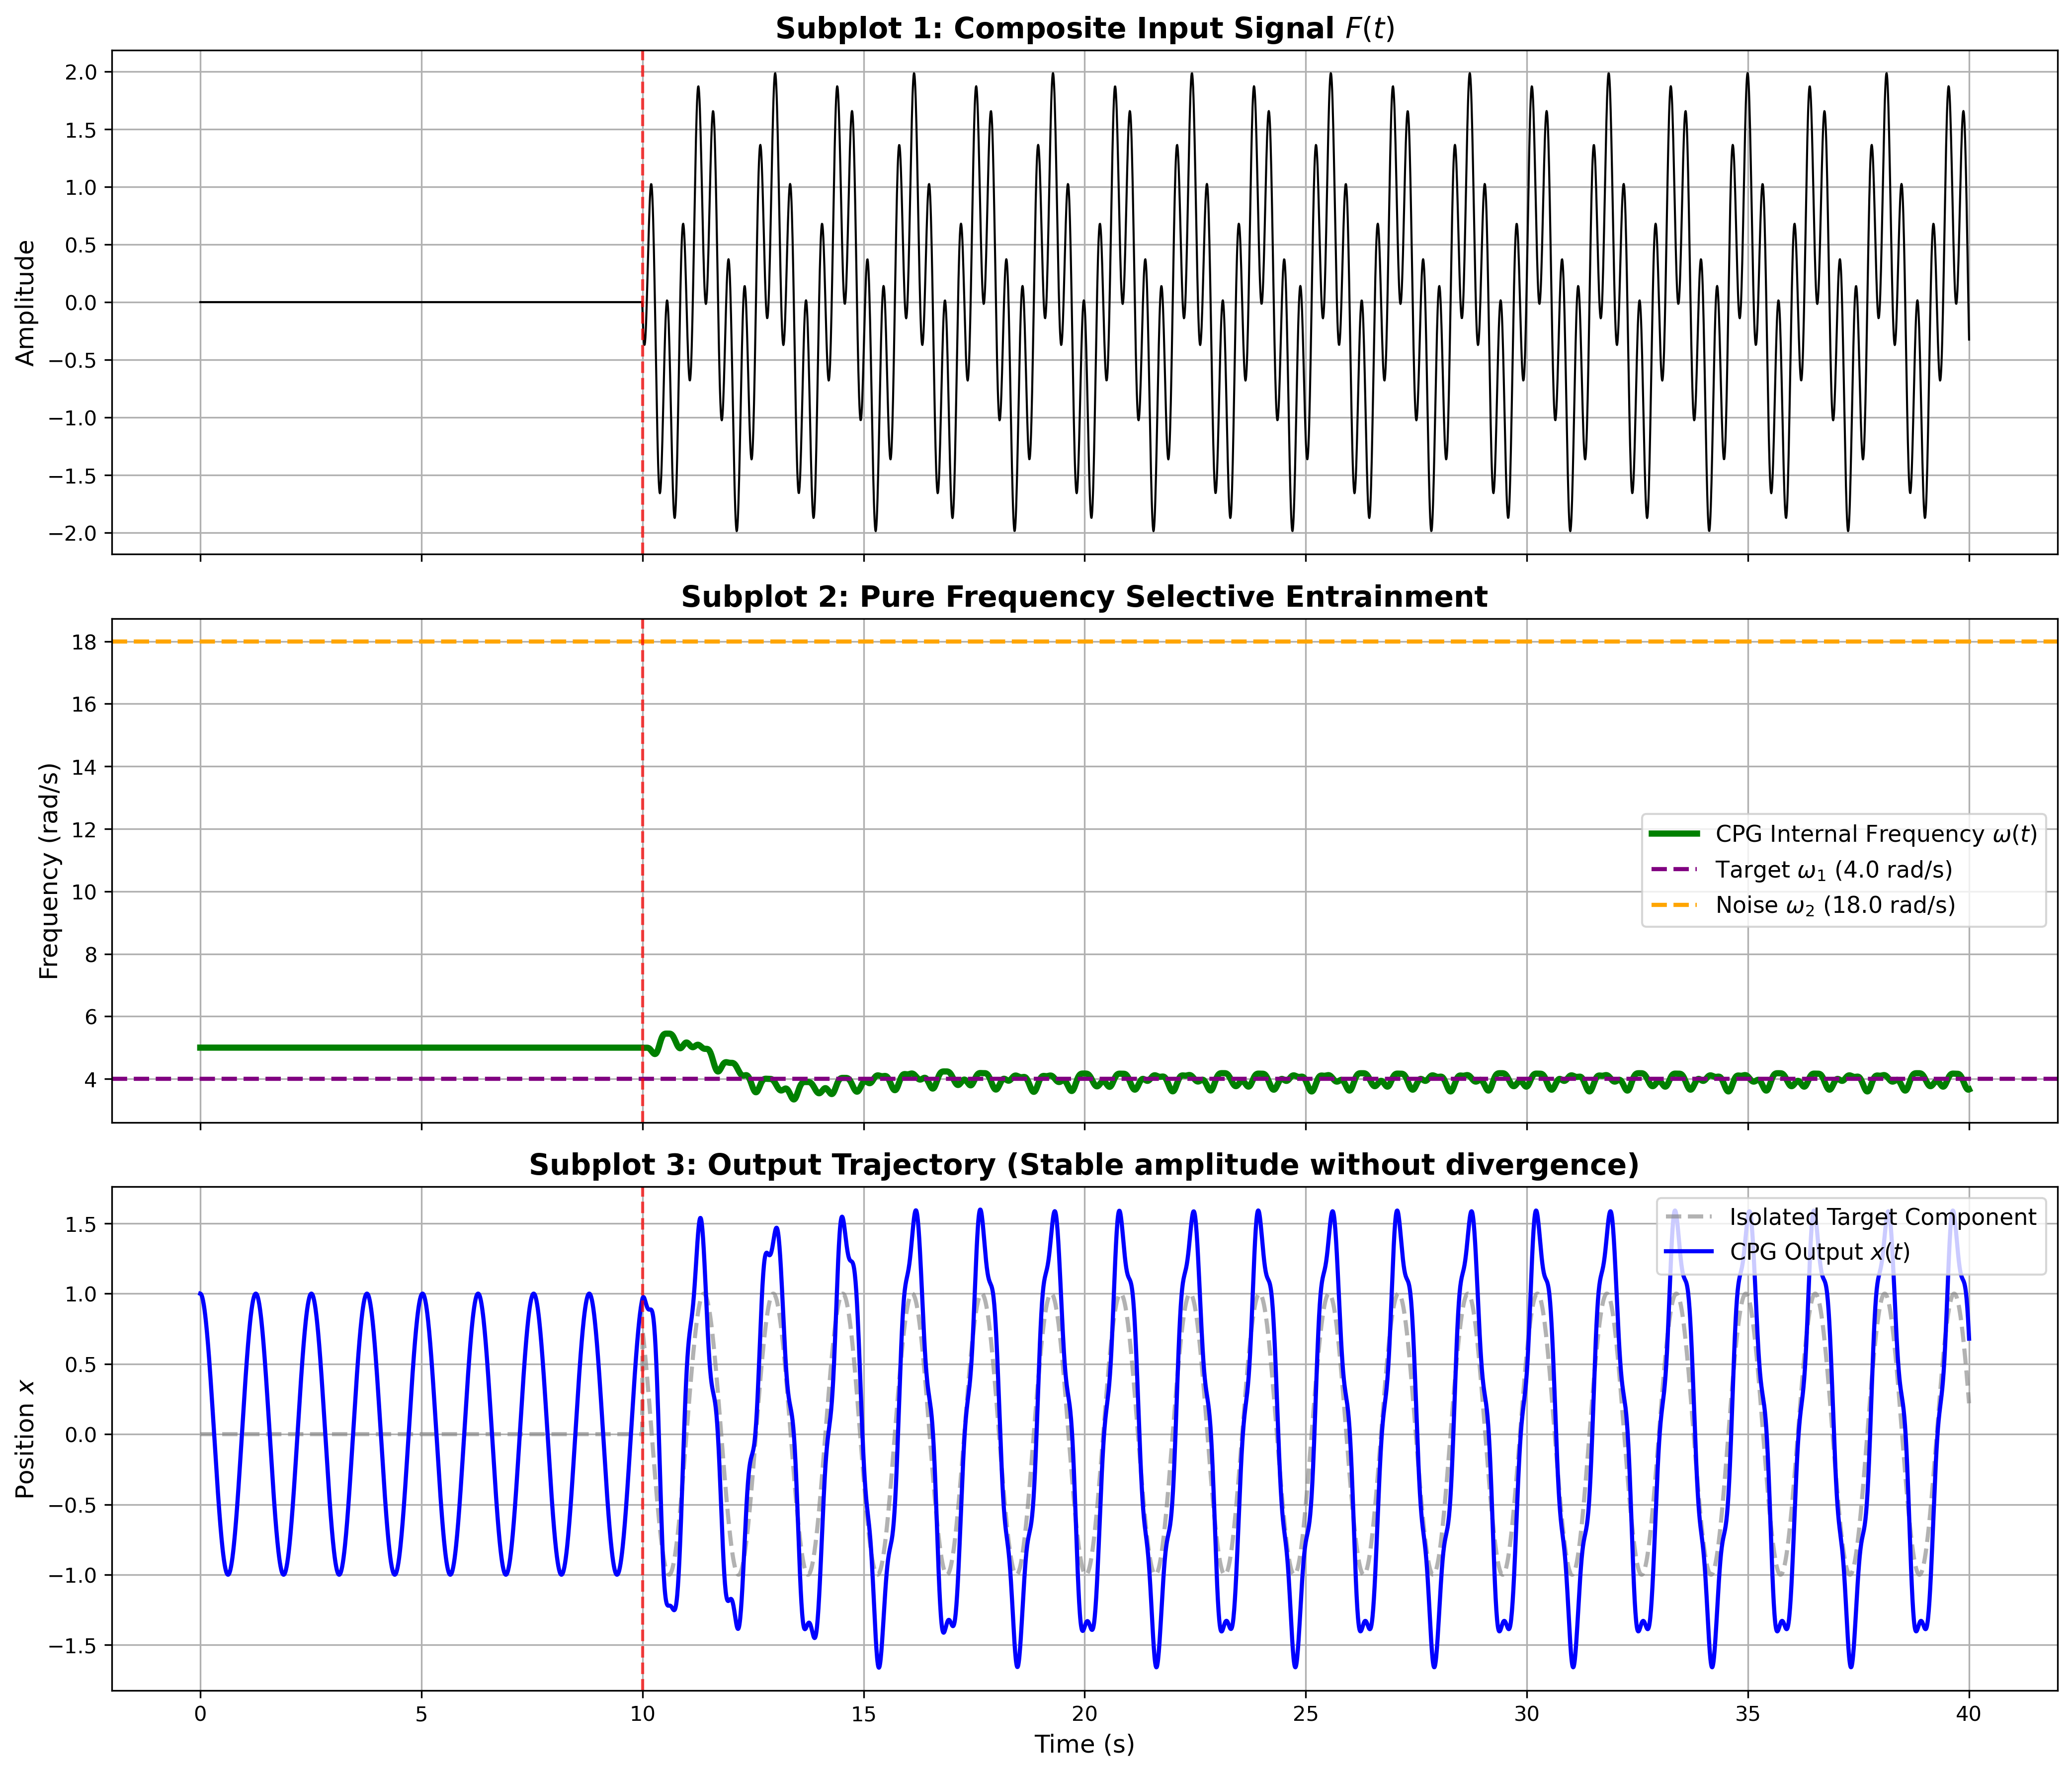
\includegraphics[width=1.0\textwidth]{figure/figure_source/muti_signal.png} 
    \caption{符合干扰信号频率下内部频率 $\omega$ 的收敛速度与稳态震荡展示}
    \label{fig:muti_signal}
\end{figure}

\section{振幅自适应（Amplitude Learning）}

将原本常数化的极限环振幅 $\mu$ 替换为一个动态学习变量 $\alpha$（代表目标振幅的平方），增加如下微分方程：
$$\dot{\alpha} = \eta F(t) \frac{x}{\sqrt{x^2 + y^2}} = \eta F(t) \cos\phi$$
\begin{itemize}
    \item $\eta$: 振幅学习率（常数）。
    \item 注意这里乘以的是 $x$（位置），而频率更新乘以的是 $y$（速度），这依然利用了正交性。
\end{itemize}
\textbf{学习结果推导：}当频率收敛且相位锁定后（$\phi = \omega_1 t - \pi/2$）：

$x(t) = r \sin(\omega_1 t)$，而 $F(t) = A_1 \sin(\omega_1 t)$。

代入振幅更新方程并取积分平均（Averaging）：
$$\langle \dot{\alpha} \rangle \approx \eta \langle A_1 \sin(\omega_1 t) \cos(\omega_1 t - \pi/2) \rangle = \eta \langle A_1 \sin^2(\omega_1 t) \rangle$$
因为 $\sin^2$ 的周期平均值是 $1/2$，所以：
$$\langle \dot{\alpha} \rangle = \frac{\eta A_1}{2}$$
只要实际振幅 $r$ 还没有追上 $A_1$，$\alpha$ 就会持续增长，直到 CPG 的输出 $x(t)$ 与输入 $F(t)$ 发生完美的动态抵消（在闭环控制架构中）。最终，CPG 的状态将完美收敛为：$$x(t) \to A_1 \sin(\omega_1 t)$$

\begin{figure}[H]
    \centering
    \includegraphics[width=1.0\textwidth]{/home/lsy/cpg_learn/Hopf/figure/figure_source/amplitude_impact.png} 
    \caption{干扰信号振幅的收敛速度与稳态震荡展示}
    \label{fig:amplitude_impact}
\end{figure}

\begin{figure}[H]
    \centering
    \includegraphics[width=1.0\textwidth]{/home/lsy/cpg_learn/Hopf/figure/figure_source/amplitude_frequency_impact.png} 
    \caption{干扰信号振幅频率同时的收敛速度与稳态震荡展示}
    \label{fig:amplitude_frequency_impact}
\end{figure}

\end{document}